\textit{Dancing Elephants} is a spectacular show in Pattaya that features $N$ elephants dancing on a line,
known as the \t{stage}.

After years of training, elephants in this show are capable of many amazing dances. The show
consists of a series of acts. In each act, exactly one elephant performs a cute dance while possibly
moving to a different position.

The show producers want to produce a photo book that contains pictures of the entire show. After each act, they want to take pictures of all elephants as seen by the spectators.

At any time during the show, multiple elephants may share the same position. In that case, they
simply stand behind one another at the same position.

A single camera can take a picture of a group of elephants if and only if all their positions lie on
some segment of length $L$ (including both its endpoints). As the elephants can spread out across
the stage, multiple cameras may be needed in order to take simultaneous snapshots of all the elephants.

As an example, suppose that $L=10$ and that the elephants are at positions $10$, $15$, $17$, and $20$ on the
stage. At this moment, a single camera can take their picture, as shown below. (Elephants are
shown as triangles; cameras are shown as trapezoids.)

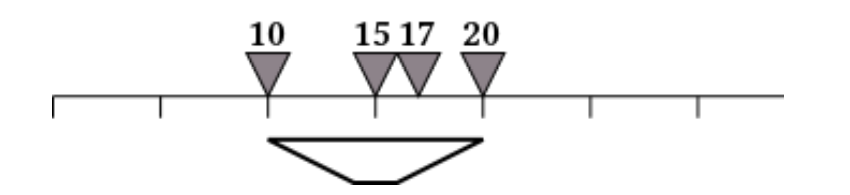
\includegraphics[bb= 0 0 100 100]{elephants3.png}

In the following act, the elephant at position $15$ dances to position $32$. After this act, we need at
least two cameras to take the snapshot.

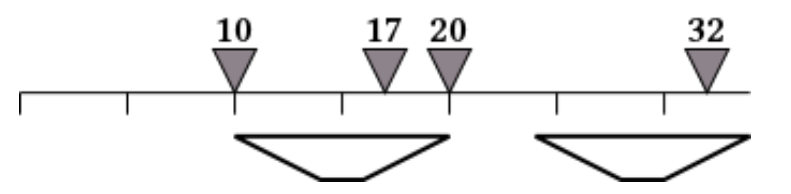
\includegraphics[bb= 0 0 100 100]{elephants2.png}

In the next act, the elephant at position $10$ moves to position $7$. For the new arrangement of elephants, we need three cameras to photograph all of them.

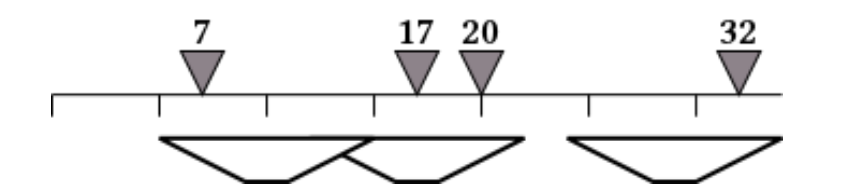
\includegraphics[bb= 0 0 100 100]{elephants1.png}

In this interactive task, you have to determine the \textit{minimum} number of cameras needed to take
the pictures after each of the acts. Note that the number of cameras needed may increase, decrease, or stay the same between acts.

Your task is to write the following procedures:

\begin{itemize}
\item Procedure \t{init(N,L,X)} that takes the following parameters:

\begin{itemize}
\item $N$~--- the number of elephants. The elephants are numbered $0$ through $N-1$.
\item $L$~--- the length of the segment captured by a single camera. You may assume
that $L$ is an integer such that $0 \le L \le 1\,000\,000\,000$.
\item $X$~--- a one-dimensional array of integers representing the initial positions of the
elephants. For $0 \le i < N$, elephant $i$ starts at the position $X[i]$. The initial
positions are in sorted order. More precisely, you may assume that
$0 \le X[0] \le \dots \le X[N-1] \le 1\,000\,000\,000$. Note that during the dance the
elephants may reorder themselves.
\end{itemize}
\end{itemize}
This procedure will be called only once, prior to all calls to \t{update}. It does not return any
value.
\begin{itemize}
\item Procedure \t{update(i,y)} that takes the following parameters:
\begin{itemize}
\item $i$~--- the number of the elephant that moves in the current act.
\item $y$~--- the position where the elephant $i$ will stand after the current act. You may assume that $y$ is an integer such that $0 \le y \le 1\,000\,000\,000$.
\end{itemize}
\end{itemize}
This procedure will be called multiple times. Each call corresponds to a single act (which
follows on from all of the previous acts). Each call must return the \textit{minimum number of cameras needed} to photograph all elephants after the corresponding act.



